\documentclass[letterpaper,12pt]{article}
\usepackage{array}
\usepackage{threeparttable}
\usepackage{geometry}
\geometry{letterpaper,tmargin=1in,bmargin=1in,lmargin=1.25in,rmargin=1.25in}
\usepackage{fancyhdr,lastpage}
\pagestyle{fancy}
\lhead{}
\chead{}
\rhead{}
\lfoot{}
\cfoot{}
\rfoot{\footnotesize\textsl{Page \thepage\ of \pageref{LastPage}}}
\renewcommand\headrulewidth{0pt}
\renewcommand\footrulewidth{0pt}
\usepackage[format=hang,font=normalsize,labelfont=bf]{caption}
\usepackage{listings}
\lstset{frame=single,
  language=Python,
  showstringspaces=false,
  columns=flexible,
  basicstyle={\small\ttfamily},
  numbers=none,
  breaklines=true,
  breakatwhitespace=true
  tabsize=3
}
\usepackage{amsmath}
\usepackage{amssymb}
\usepackage{amsthm}
\usepackage{harvard}
\usepackage{setspace}
\usepackage{float,color}
\usepackage{graphicx}
\usepackage{hyperref}
\hypersetup{colorlinks,linkcolor=red,urlcolor=blue}
\theoremstyle{definition}
\newtheorem{theorem}{Theorem}
\newtheorem{acknowledgement}[theorem]{Acknowledgement}
\newtheorem{algorithm}[theorem]{Algorithm}
\newtheorem{axiom}[theorem]{Axiom}
\newtheorem{case}[theorem]{Case}
\newtheorem{claim}[theorem]{Claim}
\newtheorem{conclusion}[theorem]{Conclusion}
\newtheorem{condition}[theorem]{Condition}
\newtheorem{conjecture}[theorem]{Conjecture}
\newtheorem{corollary}[theorem]{Corollary}
\newtheorem{criterion}[theorem]{Criterion}
\newtheorem{definition}[theorem]{Definition}
\newtheorem{derivation}{Derivation} % Number derivations on their own
\newtheorem{example}[theorem]{Example}
\newtheorem{exercise}[theorem]{Exercise}
\newtheorem{lemma}[theorem]{Lemma}
\newtheorem{notation}[theorem]{Notation}
\newtheorem{problem}[theorem]{Problem}
\newtheorem{proposition}{Proposition} % Number propositions on their own
\newtheorem{remark}[theorem]{Remark}
\newtheorem{solution}[theorem]{Solution}
\newtheorem{summary}[theorem]{Summary}
%\numberwithin{equation}{section}
\bibliographystyle{aer}
\newcommand\ve{\varepsilon}
\newcommand\boldline{\arrayrulewidth{1pt}\hline}


\begin{document}

\begin{flushleft}
  \textbf{\large{Problem Set 3}} \\
  MACS 40000, Dr. Evans \\
  Sophia Mo
\end{flushleft}

\vspace{5mm}

\noindent\textbf{Problem 1(a)}\\
The constraints for first-period consumption and first-period saving are violated.\\
\\
\noindent\textbf{Problem 1(b)}\\
The constraints for consumption in period 57, 58, 65, 66, 73, 74, and for saving in period 58, 66, 74 are violated.\\
\\
\noindent\textbf{Problem 1(c)}\\
None of the constraints is violated.\\
\\
\noindent\textbf{Problem 1(d)}\\
First, the sum of the initial guesses for each age group should be greater than zero. Second, each element in the vector should be small in magnitude because budget constraint in one period is likely to be violated if an individual saves a lot for that period. On a similar note, the difference between the guesses for savings of two consecutive age groups should be small as well; if a person saves little for the current period but a lot for the next one, her budget constraint is likely to be violated.\\
\\
\noindent\textbf{Problem 2(a)}\\
The steady-state values (all ronded to two decimal points except for the errors) are as follow:\\
\\
Savings: [0.06, 0.13, 0.19, 0.27, 0.35, 0.43, 0.52, 0.62, 0.72, 0.82, 0.94, 1.05, 1.18, 1.31, 1.45, 1.6, 1.75, 1.91, 2.08, 2.26, 2.44, 2.64, 2.84, 3.06, 3.28, 3.52, 3.76, 4.02, 4.28, 4.56, 4.85, 5.16, 5.48, 5.81, 6.15, 6.51, 6.89, 7.28, 7.68, 8.11, 8.55, 9.01, 9.49, 9.99, 10.5, 11.04, 11.6, 12.19, 12.79, 13.42, 14.08, 14.76, 15.47, 15.1, 14.72, 14.33, 13.93, 13.51, 13.08, 12.64, 12.18, 11.71, 11.23, 10.72, 10.21, 9.67, 9.12, 8.55, 7.95, 7.35, 6.72, 6.06, 5.39, 4.7, 3.98, 3.23, 2.47, 1.67, 0.85]\\
\\
Capital and Labor: 		 [ 501.94   58.4 ] \\
\\
 Wage and Interest rate: 	 [ 1.38  0.04] \\
 \\
 Consumption: 			 [1.32, 1.32, 1.32, 1.31, 1.31, 1.31, 1.31, 1.3, 1.3, 1.3, 1.3, 1.3, 1.29, 1.29, 1.29, 1.29, 1.28, 1.28, 1.28, 1.28, 1.28, 1.27, 1.27, 1.27, 1.27, 1.27, 1.26, 1.26, 1.26, 1.26, 1.26, 1.25, 1.25, 1.25, 1.25, 1.24, 1.24, 1.24, 1.24, 1.24, 1.23, 1.23, 1.23, 1.23, 1.23, 1.22, 1.22, 1.22, 1.22, 1.22, 1.21, 1.21, 1.21, 1.21, 1.21, 1.2, 1.2, 1.2, 1.2, 1.2, 1.19, 1.19, 1.19, 1.19, 1.19, 1.18, 1.18, 1.18, 1.18, 1.18, 1.17, 1.17, 1.17, 1.17, 1.17, 1.16, 1.16, 1.16, 1.16, 1.16]\\
 \\
 Aggregate consumption: 98.90\\
 \\
Euler errors:  [ -2.39727682e-11  -6.76652623e-10   1.30557332e-09  -6.15394069e-10
   4.32059388e-11  -1.50939816e-11  -1.62464486e-12   2.47574183e-12
   1.58500990e-12  -6.29496455e-14  -2.26763053e-13   7.57172103e-14
   2.24154029e-13   2.06390460e-13   1.26065824e-13   5.45674617e-14
   1.53210777e-14   6.16173779e-15   1.78745907e-14   3.99125177e-14
   6.91113833e-14   9.72000258e-14   1.26121336e-13   1.49880108e-13
   1.74305015e-13   1.93789429e-13   2.09998685e-13   2.20323759e-13
   2.29816166e-13   2.31592523e-13   2.31925590e-13   2.22821761e-13
   2.09277040e-13   1.78412840e-13   1.13464793e-13  -9.54791801e-15
  -2.25486296e-13  -5.84754467e-13  -1.10356169e-12  -1.70441439e-12
  -2.11353157e-12  -1.68909331e-12   6.01296790e-13   6.14741591e-12
   1.66853198e-11   3.52029517e-11   6.80066004e-11   9.24961219e-11
  -1.52858881e-09  -1.86461824e-09   1.54533401e-08  -2.08486499e-08
   8.57870219e-09   6.64124311e-12   2.61279332e-10  -1.70918135e-09
   4.54939864e-10   5.26712374e-09  -6.32067398e-09  -2.46639931e-10
   4.96853791e-09  -1.00058473e-09  -4.18407253e-09   5.13924681e-10
   4.43100279e-09   3.06798809e-10  -5.50990520e-09  -1.01600284e-10
   7.59131713e-09  -3.66974418e-09  -4.17030199e-09   3.41536788e-09
  -2.68450262e-10  -1.02582387e-11  -4.45754544e-13  -3.66099373e-11
   2.30068076e-10   1.25211064e-10  -3.90228072e-10]\\
   \\
Resource Constraint error:  2.13162820728e-14\\
\\
Time needed: 0.02s\\
\\
\noindent\textbf{Problem 2(b)}\\
\begin{center}
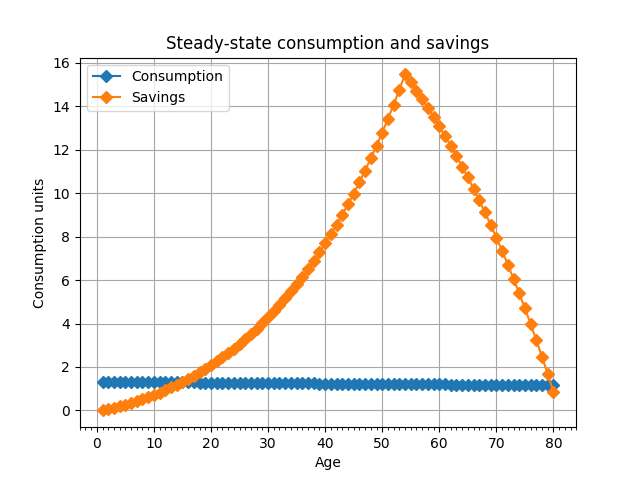
\includegraphics[scale=0.7]{ss_bc1}
\end{center}

\noindent\textbf{Problem 2(c)}\\
The new values are shown below:\\
\\
At the new steday state, capital (lifetime saving) increases because people save more to smooth consumption, given the fact that their labor income decreases earlier in life. Labor decreases because it is an exogenous variable. Wage increases and interest rate decreases because labor is now rarer (more valuable) for the firms than physical capital; the change in relative prices reflects this. Per-period savings for people aged 40 or less increase as they prepare for the earlier decrease in labor income. Consumption is less smooth than before because with the earlier start of decrese in labor income as well as a decrease in lifetime labor income, it is harder for households to smooth consumption across periods\\
\\
Savings: 			 [0.13, 0.27, 0.42, 0.59, 0.78, 0.97, 1.19, 1.41, 1.66, 1.91, 2.18, 2.47, 2.77, 3.09, 3.43, 3.78, 4.14, 4.53, 4.93, 5.34, 5.78, 6.23, 6.69, 7.18, 7.68, 8.21, 8.75, 9.3, 9.88, 10.48, 11.1, 11.73, 12.39, 13.06, 13.76, 14.47, 15.21, 15.97, 16.75, 17.55, 17.11, 16.67, 16.23, 15.79, 15.35, 14.91, 14.47, 14.03, 13.59, 13.16, 12.72, 12.29, 11.85, 11.42, 10.98, 10.55, 10.11, 9.68, 9.24, 8.81, 8.37, 7.94, 7.5, 7.07, 6.63, 6.19, 5.76, 5.32, 4.88, 4.44, 4.0, 3.56, 3.12, 2.68, 2.23, 1.79, 1.34, 0.9, 0.45] \\
\\
 Capital and Labor: 		 [ 611.27   48.  ] \\
 \\
 Wage and Interest rate: 	 [ 1.58  0.02] \\
 \\
 Consumption: 			 [1.46, 1.44, 1.43, 1.42, 1.41, 1.4, 1.39, 1.38, 1.37, 1.35, 1.34, 1.33, 1.32, 1.31, 1.3, 1.29, 1.28, 1.27, 1.26, 1.25, 1.24, 1.23, 1.22, 1.21, 1.2, 1.19, 1.18, 1.17, 1.16, 1.15, 1.15, 1.14, 1.13, 1.12, 1.11, 1.1, 1.09, 1.08, 1.07, 1.07, 1.06, 1.05, 1.04, 1.03, 1.02, 1.02, 1.01, 1.0, 0.99, 0.98, 0.98, 0.97, 0.96, 0.95, 0.95, 0.94, 0.93, 0.92, 0.92, 0.91, 0.9, 0.89, 0.89, 0.88, 0.87, 0.87, 0.86, 0.85, 0.85, 0.84, 0.83, 0.83, 0.82, 0.81, 0.81, 0.8, 0.79, 0.79, 0.78, 0.77]\\
\\
Aggregate consumption: 86.40\\
\\
\begin{center}
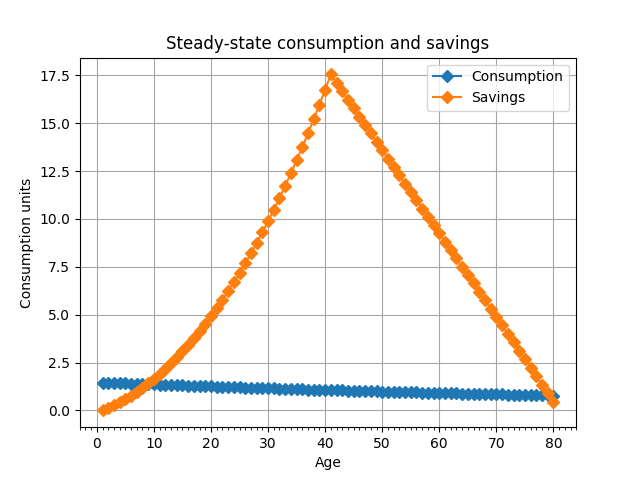
\includegraphics[scale=0.7]{ss_bc2}
\end{center}

\noindent\textbf{Problem 3(a)}\\
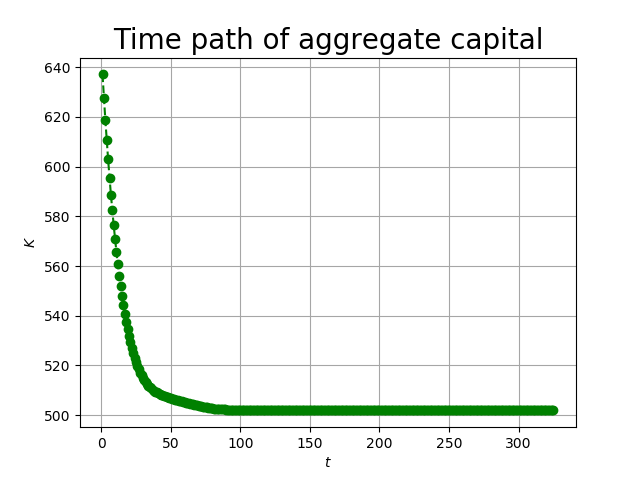
\includegraphics[scale=0.5]{kplot}
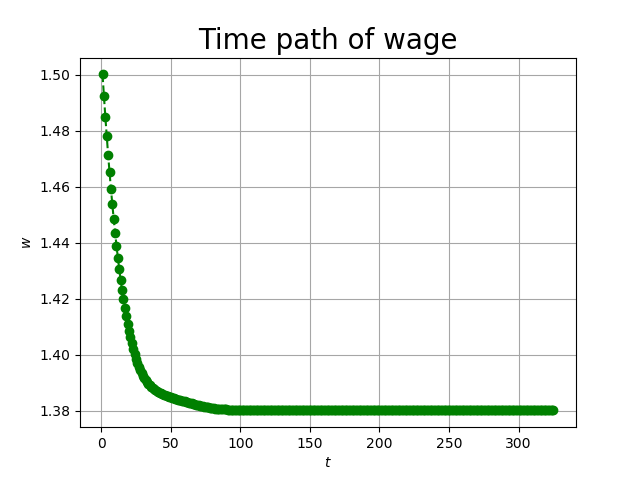
\includegraphics[scale=0.5]{wplot}
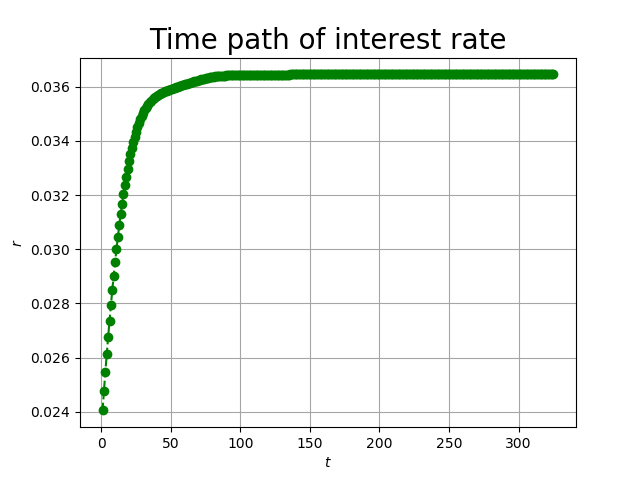
\includegraphics[scale=0.5]{rplot}
\\
\noindent\textbf{Problem 3(b)}\\
\begin{center}
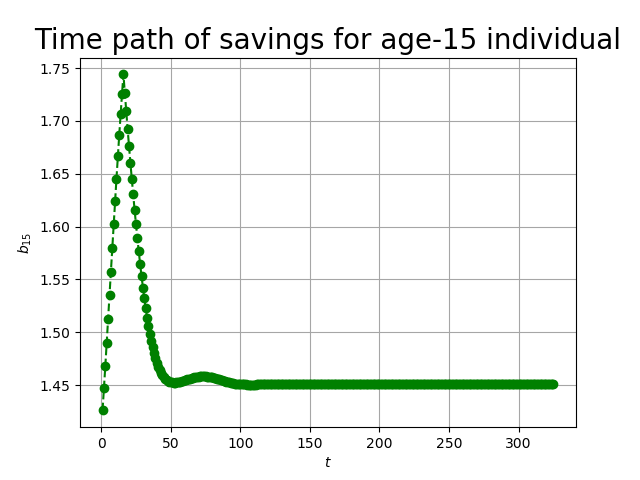
\includegraphics[scale=0.7]{bplot}
\end{center}
As seen from the graph, approximately from periods 5 to 90, the savings for age-15 individual rise above the steady-state value. Intuitively, this is because young individuals start from less than their steady-state values and it takes time for them to accumulate wealth before they could reach the savings rate given by the steady state.\\
\\
\noindent\textbf{Problem 3(c)}\\
In period 264, the economy gets to within 0.00001 of the capital steady-state level. After period 263, the aggregate capital stock never is again farther than 0.00001 away from
the steady-state.
\end{document}
